\chapter{Cluster decay in $^{294}$Og}\label{chap:294Og}

\section{Cluster emission in superheavy elements}

The region of superheavy elements, defined as the set of nuclides with $Z>104$, is an interesting one for the study of spontaneous fission because the liquid drop model predicts that all isotopes with $Z>104$ are unstable with respect to spontaneous fission. These nuclei receive additional stability due to shell effects, but they nevertheless remain short-lived and many of them will decay by spontaneous fission regardless.

Experimentally, spontaneous fission has been observed from several superheavy isotopes (those marked in green in the right panel of Figure~\ref{fig:karpovshedecay}). Other observed superheavy elements undergo a chain of several alpha decays followed by spontaneous fission. Furthermore, a variety of models predict regions where spontaneous fission dominates in the superheavy regime. One example is shown in the left panel of Figure~\ref{fig:karpovshedecay}, in which branching ratios were estimated by computing and comparing different decay lifetimes obtained from empirical formulas. Figure~\ref{fig:warda2012she} is similar, except that the spontaneous fission lifetimes were computed microscopically, as were the $Q_\alpha$ values used to estimate alpha decay lifetimes.


\begin{figure}
	\centering
	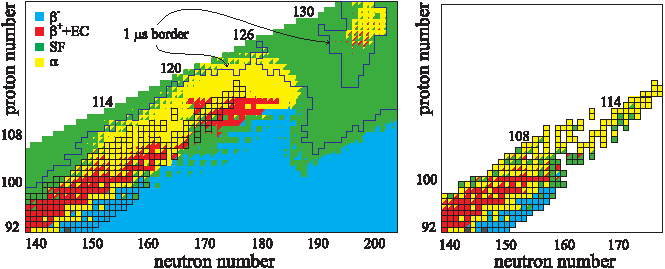
\includegraphics[width=0.9\linewidth]{TeX_files/294Og_Karpov_SHEdecay}
	\caption[Calculated (left) and experimental (right) decay modes for heavy and superheavy elements. The theoretical estimates are based on an analysis of lifetimes calculated via empirical formulae. The boxed isotopes in the left panel are those which have been measured experimentally. Isotopes falling inside the 1$\mu$s contour are predicted to live longer than 1$\mu$s. Figure adapted from~\cite{Karpova}.]{Calculated (left) and experimental (right) decay modes for heavy and superheavy elements. The theoretical estimates are based on an analysis of lifetimes calculated via empirical formulae. The boxed isotopes in the left panel are those which have been measured experimentally. Isotopes falling inside the 1$\mu$s contour are predicted to live longer than 1$\mu$s. Figure adapted from~\cite{Karpova}.}
	\label{fig:karpovshedecay}
\end{figure}


\begin{figure}
	\centering
	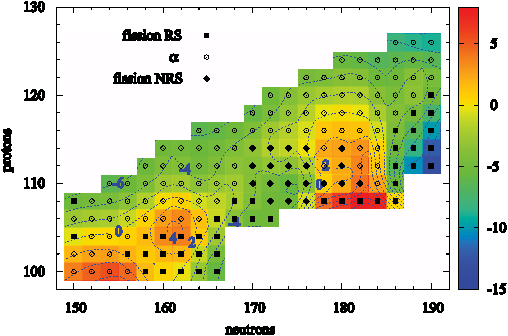
\includegraphics[width=0.7\linewidth]{TeX_files/294Og_Warda2012_SHE}
	\caption[Dominant decay modes for superheavy elements are indicated based on predictions obtained in a nuclear DFT-based framework.]{Dominant decay modes for superheavy elements are indicated based on predictions obtained in a nuclear DFT-based framework are indicated. The label ``RS'' stands for ``reflection symmetric'', meaning the least-action wavefunction at the saddle is reflection symmetric, and ``NRS'' stands for ``non-reflection symmetric.'' The colorbar indicates the predicted half-life on a logarithmic scale. Figure from~\cite{Warda2012}.}
	\label{fig:warda2012she}
\end{figure}

This still leaves open the question of fission fragments of superheavy elements, however. Several authors have predicted, using models both phenomenological~\cite{Poenaru2011, Poenaru2012, Poenaru2013, Poenaru2015, Poenaru2018,Santhosh2018, Zhang2018} and microscopic~\cite{Warda2018}, that some superheavy elements will undergo a highly-asymmetric form of fission in which the parent nucleus decays into two fragments, with the heavy fragment near the doubly-magic nucleus {\Pb}. This particular decay mode is significant enough to have earned its own name in the literature, where it is known variously as cluster emission, cluster radioactivity, or lead radioactivity~\cite{Sandulescu1980,Poenaru1986,Royer1998,Poenaru2010,Warda2011}. The phenomenon of cluster emission was first observed in 1984 in the decay $^{223}$Ra$\rightarrow$$^{209}$Pb + $^{14}$C~\cite{Rose1984} and has since been observed in several actinides. In all cases seen so far, it is a rare event with a small branching ratio~\cite{Poenaru2010}.

The mechanism of cluster emission is based on the stability of the doubly-magic nucleus {\Pb}. {\Og} is a particularly excellent candidate for cluster emission because the cluster it is predicted to emit, {\Kr}, receives additional stability due to its having a magic number of neutrons.  Semiempirical arguments based on the nuclear symmetry energy lend additional support to this candidate, since {\Og} and {\Pb} have a similar $N/Z$ ratio~\cite{Warda2018}.

We took this prediction one step further by calculating the full spontaneous fission fragment distribution of {\Og} using a microscopic approach. As will be shown, the distribution is sharply-peaked around {\Pb}, and this will be shown to be quite robust with respect to various inputs. A visualization of the process using the nucleon localization function shows strong evidence of a {\Pb} prefragment being formed early in the post-saddle stage of the evolution.

\section{Predicted spontaneous fission yields of $^{294}$Og}

Potential energy surfaces were computed for each of three EDFs: \hfb~\cite{Schunck2015}, a Skyrme functional which was optimized to data for spherical and deformed nuclei, including fission isomers; SkM*~\cite{Bartel1982}, another Skyrme functional designed for fission barriers and surface energy; and D1S~\cite{Berger1989}, a parameterization of the finite-range Gogny interaction fitted on fission barriers of actinides. A comparison of the different PESs as a function of multipole moments $Q_{20}$ and $Q_{30}$ is shown in Figure~\ref{fig:294ogthreepes}. Despite the quantitative differences between the functionals, one can see that the surfaces strongly resemble one another. Some common features we highlight are: a symmetric saddle point occurring around $Q_{20}\approx 40$\,b; a second barrier beginning around $Q_{20}\approx100-120$\,b along the symmetric fission path; the presence of local minima at large deformations (marked by stars in the figure); a deep valley that leads to an highly-asymmetric split; and a secondary, less-asymmetric fission valley that emerges at large elongations.


\begin{figure}
	\centering
	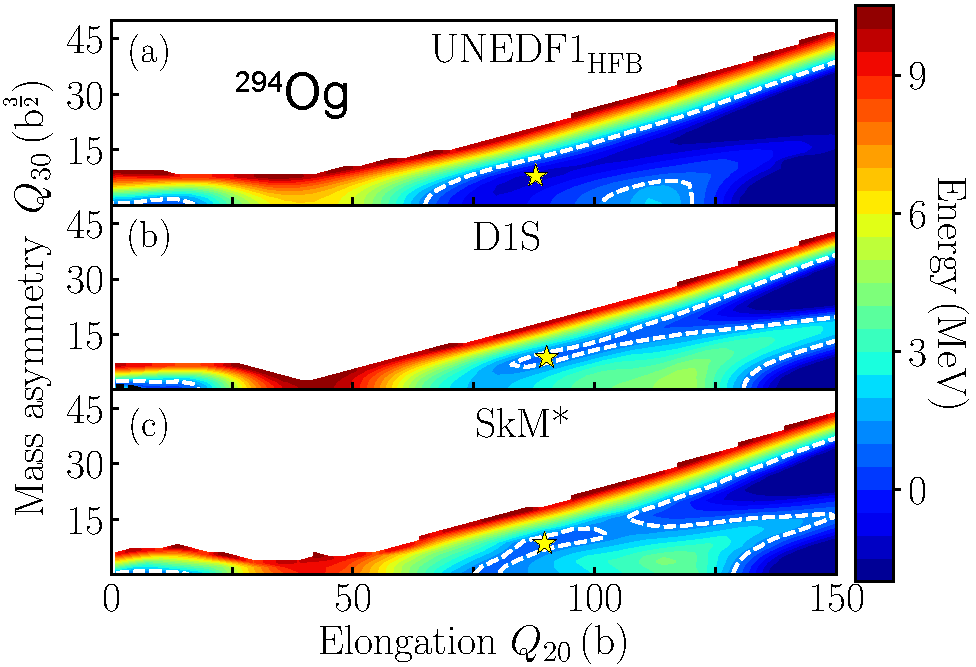
\includegraphics[width=0.7\linewidth]{TeX_files/294Og_three_PES}
	\caption[PES comparison for $^{294}$Og using EDFs {\hfb}, D1S, and SkM*.]{Comparison of the PESs for \Og{} in the $(Q_{20},Q_{30})$ collective plane obtained in \hfb{} (a), D1S (b), and SkM* (c) EDFs. The ground-state energy $E_{gs}$ is normalized to zero. The dotted line in each figure corresponds to $E_0-E_{gs}=1$\,MeV, which was used to determine the inner and outer turning points. The local energy minima at large deformations are marked by stars.}
	\label{fig:294ogthreepes}
\end{figure}

%% This passage is lifted straight from the paper, FYI
But there are differences as well, such as the height of the first saddle point, the depth of the highly-asymmetric fission valley, and the height of the ridge separating the two fission valleys. As a result, the outer turning points are pushed to larger elongations in D1S and SkM* as compared to \hfb{}. These differences in the PES topography strongly affect the predicted spontaneous fission half-lives $\tau_\mathrm{SF}$, which in the case of \hfb{}, SkM* and D1S are $9.1\times10^{-9}\,$s, $4.0\times10^{-5}\,$s and $3.2\times10^{-2}\,$s, respectively (see also~\cite{Staszczak2013,Baran2015} for a detailed discussion of half-lives). These large variations of $\tau_\mathrm{SF}$ reflect the well-known exponential sensitivity of spontaneous fission half-lives to changes in the quantities entering the collective action~\eqref{eq:action}. The $\tau_\mathrm{SF}$ predictions of \hfb{} and, to a lesser degree,  SkM* are incompatible with experiment, as $^{294}$Og  is known to  decay by $\alpha$-decay with a half-life of 0.58\,ms~\cite{Brewer2018}. The D1S result should not be taken too seriously, either, since they were performed in a smaller collective space leading to overestimation of the half-lives~\cite{Giuliani2014,Sadhukhan2014}.

It is to be noted that while half-lives are very sensitive to details of the calculations, the models used here are very consistent with each other and with experiment when it comes to global observables, such as alpha-decay energies, deformations, and radii~\cite{Heenen2015,Giuliani2019}. It will be demonstrated below that spontaneous-fission mass and charge yields are also robustly predicted (though experimental confirmation has not yet occurred). This robustness will be shown by varying the EDF, the collective space, the collective inertia, and the strength of the Langevin dissipation tensor (recall Section~\ref{sect:fissionmethod}).
%% End of lifted passage

The EDF and the collective space were varied together; a different collective space was used for each EDF in the tunneling portion of the PES. The {\hfb} calculation was carried out in a four-dimensional collective space consisting of the collective coordinates $(Q_{20}, Q_{30}, Q_{22}, \lambda_2)$. By examining this PES, we were able to reduce the dimensionality of the PES for the other two functionals. The SkM* calculation was performed in a piecewise-continuous space. Between the ground state and the isomer state, $Q_{30}$ does not play a significant role and so the system was described using  $(Q_{20}, Q_{22}, \lambda_2)$. Likewise, $Q_{22} \approx 0$ once the isomer state is reached and reflection symmetry is broken ($Q_{30} \neq 0$), suggesting use of the coordinates  $(Q_{20}, Q_{30}, \lambda_2)$. Finally, for the functional D1S we decided to see how our yields would be affected if we did not consider dynamical pairing fluctuations or axial symmetry breaking at all, which results in a drastic reduction to computation time. Those calculations were performed in the collective space $(Q_{20}, Q_{30})$.

In the region of Langevin dynamics, we found again that $Q_{22} \approx 0$. Consequently, this region was limited to two dimensions $(Q_{20}, Q_{30})$ in all cases.

\begin{figure}
	\centering
	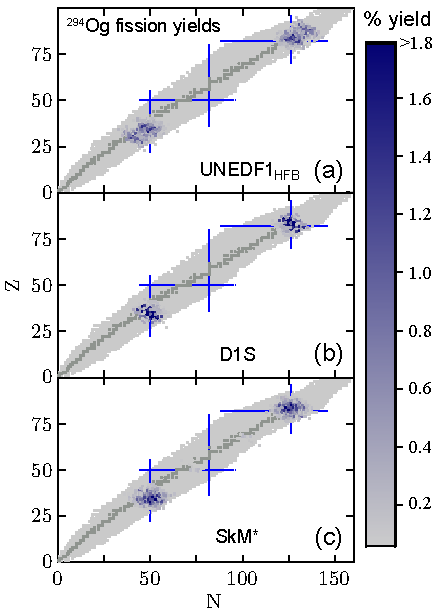
\includegraphics[width=0.9\linewidth]{TeX_files/294Og_3yields}
	\caption[N-Z fission fragment yields from $^{294}$Og]{Fission fragment distributions for \Og{} obtained in \hfb{} (a), D1S (b), and SkM* (c) EDFs using the non-perturbative cranking ATDHFB inertia and  the baseline  dissipation tensor $\mathbf{\eta}_0 = (\eta_{11},\eta_{22},\eta_{12}) = (50\hbar,40\hbar,5\hbar)$. Known isotopes are marked in gray~\cite{NuDat}. Magic numbers 50, 82, and 126 are indicated by dotted lines.}
	\label{fig:294og3yields}
\end{figure}

The resulting yields are shown in Figure~\ref{fig:294og3yields} as a function of $Z$ and $N$. As expected, the yields are peaked in the region of {\Pb} with a sharp fall-off. Likewise, the projected distributions onto the mass and charge axes show a clear preference for cluster emission, regardless of functional, as seen in the top panels of Figure~\ref{fig:294ogcompareall}.

\begin{figure}
	\centering
	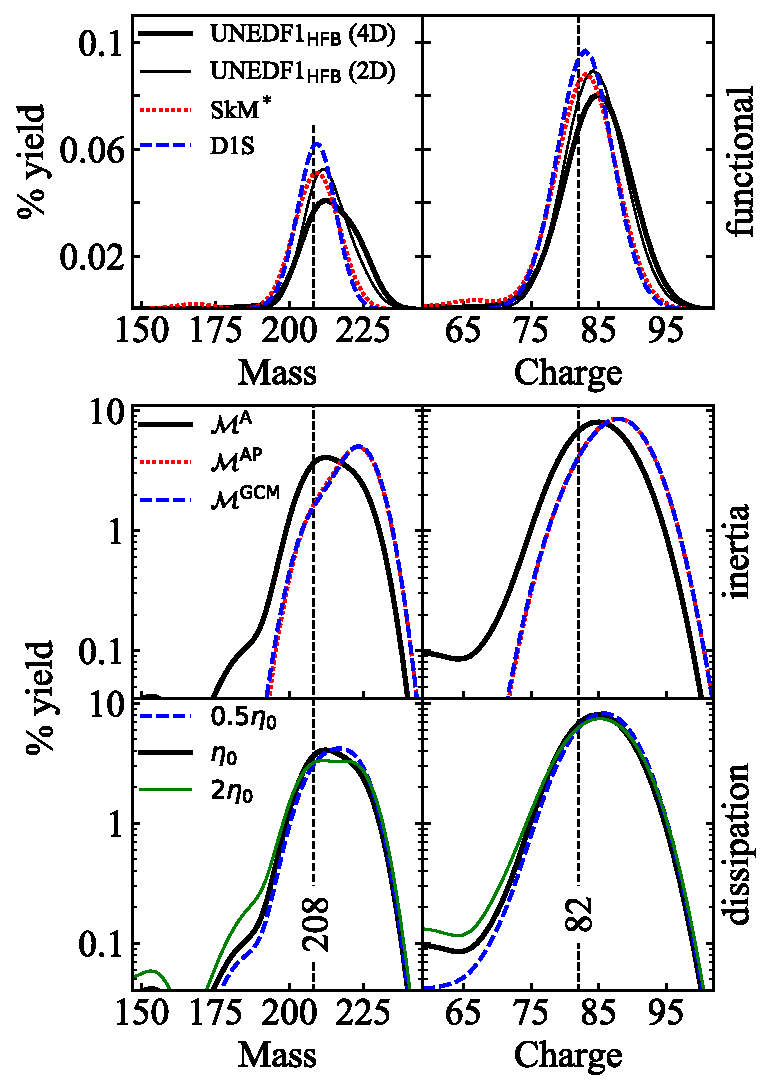
\includegraphics[width=0.7\linewidth]{TeX_files/294Og_compare_all}
	\caption[$^{294}$Og heavy fragment masses and charges.]{Upper panel: Predicted heavy fragment mass (left) and charge (right) yields of \Og{} using different functionals (top, linear scale). Lower panels: collective inertias (middle, logarithmic scale) and dissipation tensor strengths (bottom, logarithmic scale). The baseline calculation was performed using the \hfb{} functional in a 4D space with non-perturbative cranking ATDHFB inertia and dissipation tensor strength $\mathbf{\eta}_0$.}
	\label{fig:294ogcompareall}
\end{figure}

As discussed in Chapter~\ref{chap:Model}, the collective inertia can also have a large impact on the fission dynamics. Using the {\hfb} functional, we compared our result with the non-perturbative cranking ATDHFB inertia, {\MATDHF}, to two other expressions for the inertia which are computationally less expensive to compute and therefore commonly-used in large-scale calculations: the perturbative ATDHFB inertia {\MATDHFp} (which appears smoothed-out compared to {\MATDHF}~\cite{giuliani2018b}), and the perturbative GCM inertia {\MGCMp} (which is smooth and also lower in magnitude than {\MATDHF} or {\MATDHFp} by roughly a factor of 1.5~\cite{giuliani2018b}). The result, shown in the middle panels of Figure~\ref{fig:294ogcompareall}, show that the distribution has shifted slightly, but that {\MATDHFp} and {\MGCMp} give identical, or nearly-identical results to one another. The smoothness of the perturbative inertias apparently allow fluctuations to drive the system to more extreme fragment configurations. This suggests that the magnitude of the inertia matters less than the topography for computing fission yields (though we note that this would not be true for calculating half-lives, which depend exponentially on the magnitude of the inertia).

We also vary the strength of dissipation tensor by adjusting the parameter $\mathbf{\eta}$. Our starting point $\mathbf{\eta}_0 = (\eta_{11},\eta_{22},\eta_{12}) = (50\hbar,40\hbar,5\hbar)$ is taken from~\cite{Sadhukhan2016}, where it was obtained by adjusting $\mathbf{\eta}$ to match the experimental fragment distribution of $^{240}$Pu. Shown in the bottom panels of Figure~\ref{fig:294ogcompareall}, we find that fluctuations do not affect the peak of the distribution, consistent with the results of~\cite{Randrup2011,Sierk2017,Sadhukhan2017}. The primary effect is in the tails, suggesting that fluctuations affect only a relatively-small number of nucleons.

\section{Fragment formation in $^{294}$Og}\label{sect:294Ogfrags}

The Langevin dynamics approach is useful for calculating fragment yield distributions, but it does not offer much physical insight into the process of fragment formation. In order to better understand fragment formation for the most-probable fragments, we computed the nucleon localization function (section~\ref{sect:locali} and References~\cite{Zhang2016,Sadhukhan2017}) along the cluster emission path. This is shown in Figure~\ref{fig:294oglocali}, where it is compared to the spherical fragments {\Pb} and {\Kr}. We found that the lead prefragment is well-localized just outside the outer turning line. The $N\approx50$ neutrons belonging to krypton are also well-localized at early stages of the evolution, but the $Z\approx36$ protons are not, highlighting the importance of shell closures in prefragment formation.

\begin{figure}
	\centering
	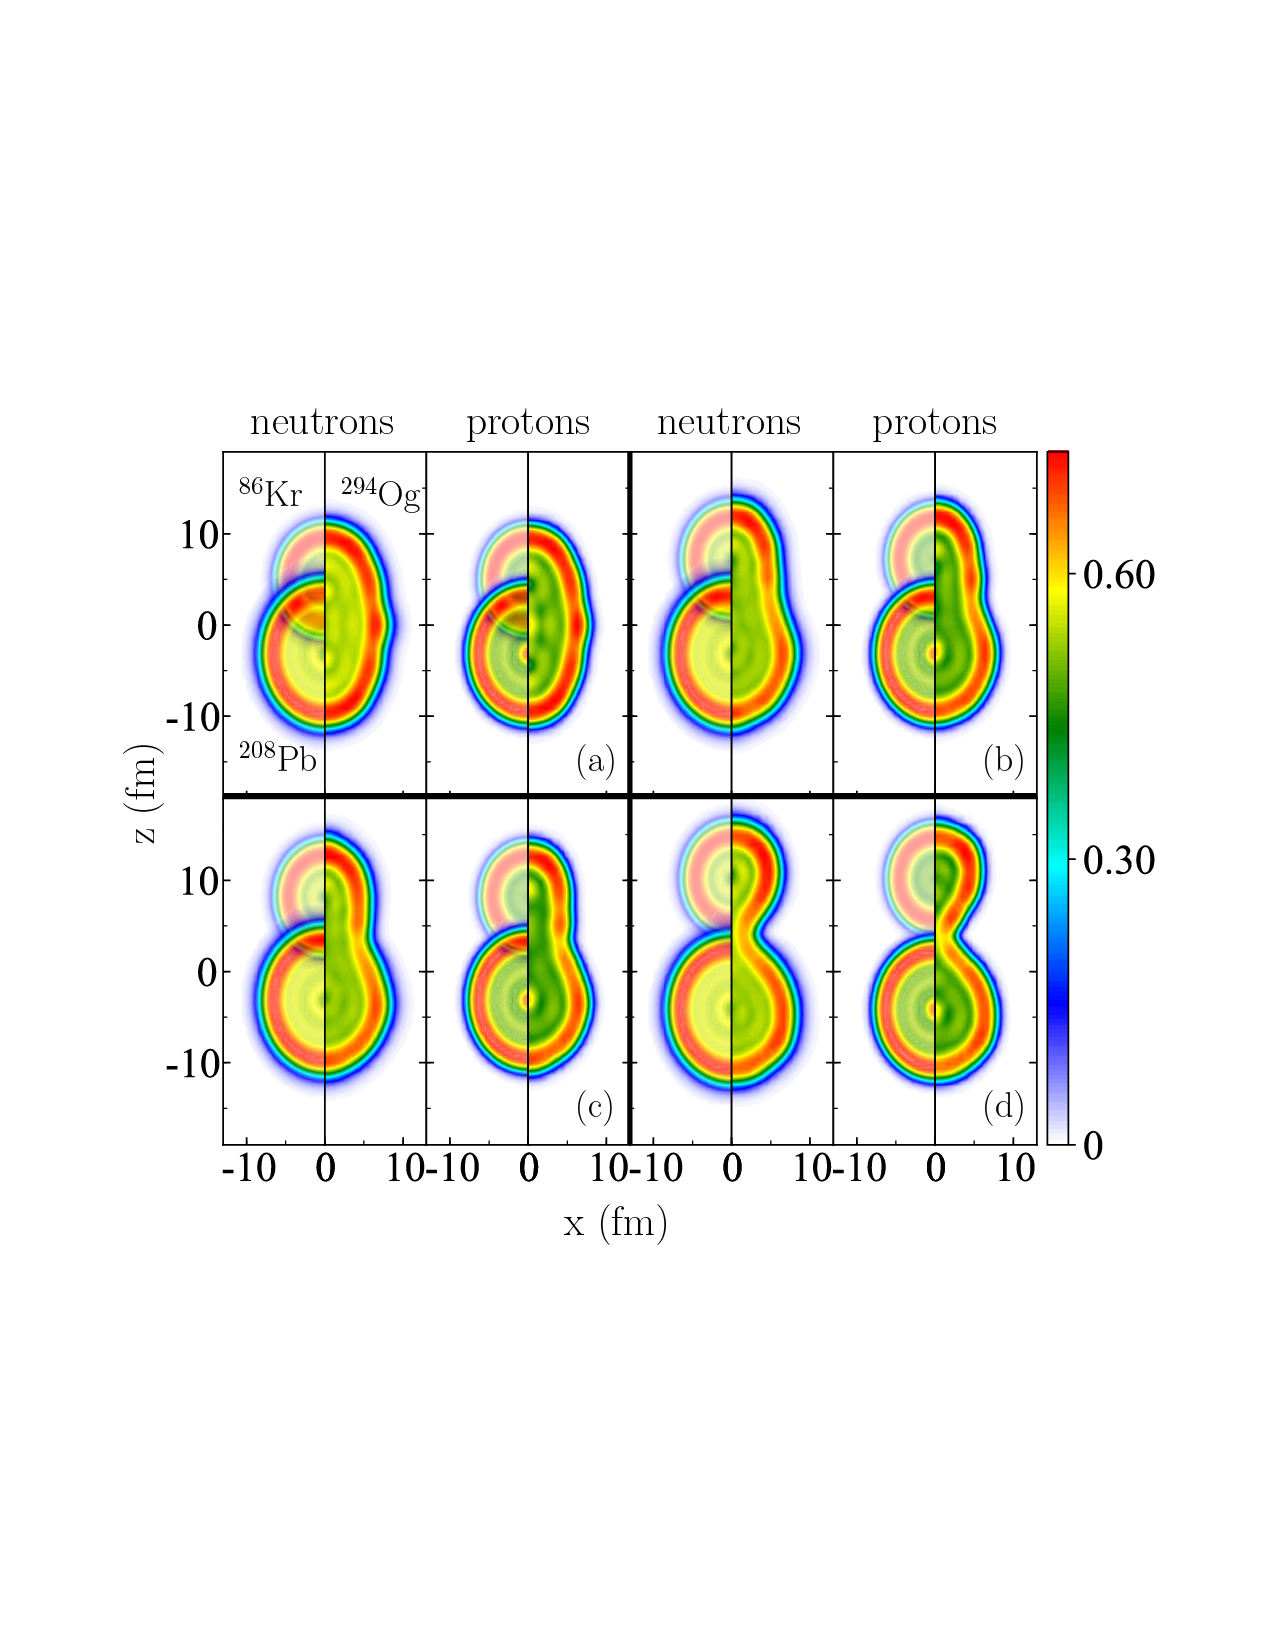
\includegraphics[width=0.9\linewidth]{TeX_files/294Og_locali}
	\caption[Nucleon localization visualization of $^{294}$Og prefragment formation.]{Nucleon localization functions for several deformed configurations of {\Og}. For comparison, localizations are also shown for the fragments {\Pb} and {\Kr} on the left side of each subplot. The configurations shown correspond to Fig. 1 from the paper, with multipole moments $(Q_{20}, Q_{30})=$ (a) (75\,b, 0); (b) (120\,b, 17\,$\mathrm{b}^\frac{3}{2}$) [${\sim}$OTL]; (c) (140\,b, 24\,$\mathrm{b}^\frac{3}{2}$); and (d) (264\,b, 60\,$\mathrm{b}^\frac{3}{2}$) [${\sim}$scission].}
	\label{fig:294oglocali}
\end{figure}

%If this is a general result, one could leverage this insight to predict fission fragments as early as the outer turning line, resulting in a major reduction in total computing time because of the reduced PES. A method which exploits this possibility is described in Appendix~\ref{append:Fragments}. % But this might have to move up, depending how the r-process calculations go


\section{Experimental search for cluster emission in $^{294}$Og}
%Perhaps the biggest uncertainty we'll see, or the biggest deviation from experiment, will be the distribution width. That's because we folded our Langevin results with a Gaussian function, the width of which was chosen rather arbitrarily to be $\sigma_A=6, \sigma_Z=4$. The values used in $^{240}$Pu were 3 and 2, but the $Q_N$ value they used to define scission was quite a bit smaller too. Since we had a much larger $Q_N$ cutoff, we needed to account for larger particle number fluctuations. But these numbers were just kind of arbitrary. I'm not too worried about this because the peak is the part that matters, and we clearly saw a peak at the cluster location.

The effort to detect cluster emission from superheavy elements is underway. However, one of the biggest challenges standing in the way of observation of cluster emission from {\Og} is the problem of statistics. There have only been 5 recorded instances of {\Og}, from the first observations in 2005~\cite{Oganessian2006} to the most recent in 2018~\cite{Brewer2018}.\footnote{In fact, there were reports as early as 2004~\cite{Oganessian2004} that fission fragments resulting from the spontaneous fission of {\Og} may have been detected, but these are unconfirmed.} To maximize the possibility of detecting spontaneous fission events as they happen, there is some discussion in the experimental community about building an ionization chamber for superheavy element research with the ability to distinguish fragments by their Z-value. This is discussed at some length in~\cite{Brewer2018}.

%``Among these SF events, there were signals correlated with incoming recoil-like signals within the time range of the {\Og} half-life. We have inspected the possible assignment of some SF events to the fission of {\Og}. In the past, as well very recently, {\Og} was considered as a system consisting of doubly magic {\Pb} and singly magic N = 50, {\Kr}. These two components are well bound stable nuclei. One can envision that an asymmetric fission of {\Og} into {\Pb} and {\Kr} fragments might be somewhat enhanced.
%
%``However, especially since the decay time of {\Og} is not sufficiently different from $^{258}$No decay, one cannot make an assignment to {\Og} activity based only on the half-life of SF events. The energy of SF events vary, since we detect sometimes only a partial energy of fission fragments. Such events are more likely to arise from the SF activity produced in a multinucleon transfer involving the Cf isotope in the target. The indistinguishability of complete-fusion from transfer reaction products provides motivation for an ionization chamber, which would have a discrimination capability for the atomic number Z, placed before the implantation Si counter. Construction and anticipated performance of such an ionization chamber based on gas electron multiplier (GEM) technology was recently discussed...''